\chapter{Proposed Method}
\label{chap:proposed}
\section{Overview}
   %input output only melodic constrains
   %flow chart
      \begin{figure*}[tp]
         \begin{center}
            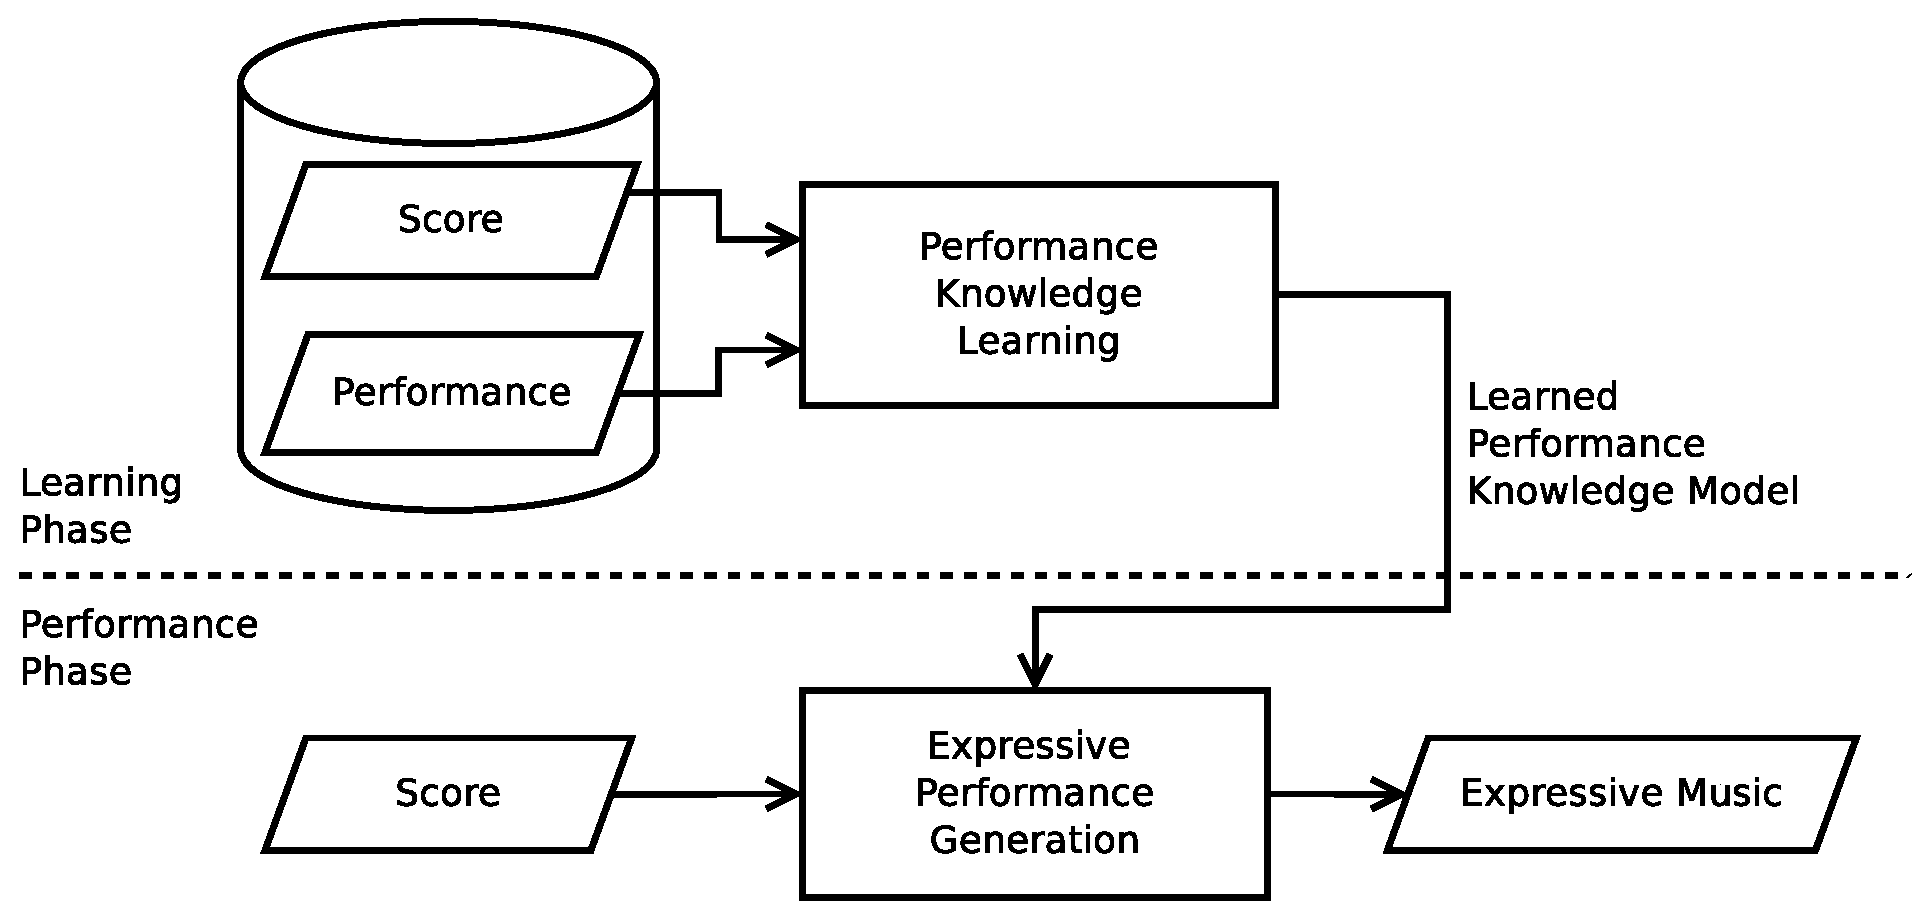
\includegraphics[width=\textwidth]{fig/high_lev_arch}
         \end{center}
         \caption{High-level system architecture} 
         \label{fig:flow}
      \end{figure*}
The high-level architecture of the purposed system is shown in Fig. \ref{fig:flow}. The system has two phases, the upper half of the figure is the learning phase, the lower half is the performing phase. In the training phase, score and expressive performance recording pairs, split into phrases by human, are used as training examples for structural support vector machine with hidden Markov model output (SVM-HMM) algorithm to learn performance knowledge model. In the performing phase, a score will be given to the system for expressive performance. The SVM-HMM generation module will use the performance knowledge learned in the previous phase to produce expressive performance. The SVM-HMM output then go through a MIDI generator and MIDI synthesizer to produce audible performance.
%TODO: refer to feature exction and corpus chapter

All the scores and recordings are monophonic and contains only one musical phrase. The phrasing is done by human, thus the system is a semi-automatic system. The learning algorithm, namely SVM-HMM, can only perform off-line learning, so the learning phase can only work in a non-realtime scenario. The generating phase can work much faster, expressive music can be generated almost instantaneously. 

There are many ways the user can control the performance style of the final output: first, the user can choose the training corpus. Theoratically, a set of samples from a single performer can generate a model which capture his/her style. Second, the phrasing of a song is given by the user. Since phrasing controls the overall structural interpretation of a music piece, the user is given indirect control over the performance style.


In the following sections, we will walk through the detail steps in the learning and performing phases, and some implementation detail. The features used will be presented in the end of this chapter.


%TODO: START COPY-PASTE
%\chapter{Theoretical Background}
%\framebox{REVIEW1}
\section{A Brief Introduction to SVM-HMM}
\label{sec:svm-hmm}
In this thesis, we use structural support vector machine to learn performance knowledge from expressive performance samples. Unlike traditional SVM algorithm, which can only produce univariate prediction, structural SVM can produce structural predictions like tree, graph or sequence. Structural SVM with hidden Markov model output (SVM-HMM) has been successfully applied to part-of-speech tagging problem\cite{svm2009}. The part-of-speech tagging problem has some similarity with expressive performance problem. In part-of-speech tagging, one tries to identify the role by which the word plays in the sentence, while in expressive performance, one tries to determine how a note should be played, usually based on it's role in the musical phrase. %For example, an authentic cadence at the end of a phrase is usually played louder and stronger than a embellishment note in the middle of a phrase. 
Thus, we believe SVM-HMM will be a good candidate for expressive performance. The following introduction and formulas relies heavily on \cite{svm2009, svm2005, svm2003}.

%Ref: 20130420 slides

%TODO:discuss traditional SVM here?
Traditional SVM prediction problem can be described as finding a function 
$$h: \mathcal{X \rightarrow Y}$$ with lowest prediction error. $\mathcal{X}$ is the input features space, and $\mathcal{Y}$ is the prediction space. In traditional SVM, elements in $\mathcal{Y}$ are labels (classification) or real values (regression). But structural SVM extends the framework to generate structural output, such as tree, graph or sequence.
To extend SVM to support structured output, the problem is modified as finding a discriminant function $$F: \mathcal{X} \times \mathcal{Y} \rightarrow \mathcal{R}$$, in which the input/output pairs are mapped to a real number score. To predict an output $y$ for an input $x$, one try to maximize $F$ over all $y \in \mathcal{Y}$. 

$$f(x) = \argmax_{y\in\mathcal{Y}} F(w,x,y)$$

Let $F$ be a linear function of the form:

$$ F = \mathbf{w}^{T}\Psi(x,y)$$, 
where $\mathbf{w}$ is the parameter vector, and $\Psi(x,y)$ is the kernel function relating input $x$ to output $y$. $\Psi$ can be defined to accommodate various kind of structures. 

%emprical risk
For each structure we want to predict, a loss function that measures the accuracy of of a prediction is required. A loss function $\Delta:\mathcal{Y}\times\mathcal{Y}\rightarrow R$ need to satisfy the following property:

$$\Delta(y, y') \geq 0 \ for\ y \neq y'$$
$$\Delta(y, y) = 0 $$

The loss function is assumed to be bounded. Let's assume the input-output pair $(x,y)$ is drawn from a join distribution P(x,y), the prediction problem is to minimize the total loss:

%TODO: total loss formula 2005 sec 2.1
$$R_p^\Delta = \int_{\mathcal{X} \times \mathcal{Y}} \Delta (y, f(x))dP(x,y)$$

Since we can't directly find the distribution $P$, we need to replace this total loss with a empirical loss, which can be calculated from the observed training set of $(x_i, y_i)$ pairs.
%TODO: emprical loss
$$R_s^\Delta(f) = \frac{1}{n}\sum^n_{i=1}\Delta(y_i, f(x_i))$$

Now we are ready to extend SVM to structural output, starting with a linear separable case, and we will then extend it to soft-margin formulation. 

A linear separable case can be expressed by a set of linear constrains
%TODO: 2005 formula 4
$$\forall i \in \{1,\cdots,n\}, \forall \hat{y_i}\in\mathcal{Y}: \mathbf{w}^T [\Psi(x_i, y_i) - \Psi(x_i, \hat{y_i})]\geq 0$$

The constrains imply that the groundtruth $y_i$ for $x_i$ has the minimum $F$ value than any other $\hat{y}_i \neq {y_i}$.

The key concept of SVM is the large margin principle. We not only want to find a solution that statisfies the constrains, but also we want to maximize the margin between the groundtruth and the second best $\hat{y}_i$:
%TODO: 2005 formula 4+
$$
\begin{aligned}
& \max_{\gamma, \mathbf{w}:\|\mathbf{w}\| = 1} \gamma \\
& s.t \; \forall i \in \{1,\cdots,n\}, \forall \hat{y_i} \in\mathcal{Y}: \mathbf{w}^T [\Psi(x_i, y_i) - \Psi(x_i, \hat{y_i})] \geq \gamma\\
\end{aligned}
$$

, which is equivalent to the convex quadratic programming problem:
%TODO: 2005 formula 5,k 6
$$
\begin{aligned}
   & \min_{\mathbf{w}, \xi_i \geq 0} \frac{1}{2}\|\mathbf{w}\|^2 \\\
    &s.t.\; \forall i \in \{1,\cdots,n\},\hat{y_i} \in \mathcal{Y}: \mathbf{w}^T[\Psi(x_i,y_i) - \Psi(x_i,\hat{y_i})] \geq 1\\
\end{aligned}
$$

To extend the linear-separable case to non-separable case, slack variables $\xi_i$ can be introduced to penalize prediction errors, results in a soft-margin formalization:
%TODO: 2005 formula SVM1
$$
\begin{aligned}
   & \min_{\mathbf{w}, \xi_i \geq 0} \frac{1}{2}\|\mathbf{w}\|^2 + \frac{C}{n}\sum^n_{i=1}\xi_i\\
    &s.t.\; \forall i \in \{1,\cdots,n\},\hat{y_i} \in \mathcal{Y}: \mathbf{w}^T[\Psi(x_i,y_i) - \Psi(x_i,\hat{y_i})] \geq 1 - \xi_i \\
\end{aligned}
$$

$C$ is the weighting parameter controlling the trade-off between low training error and large margin. The optimal $C$ varies between different problems, so experiment should be conducted to find the optimal $C$ for our problem.

Intuitively, a constrain violation with larger loss should be penalize more than the one with smaller loss. So I. Tsochantaridis et al. \cite{svm2005} proposed two possible way to take the loss function into account. The first way is to re-scale the slack variable by the inverse of the loss, so a high loss leads to smaller re-scaled slack variable:
%slack rescaling

$$
\begin{aligned}
   & \min_{\mathbf{w}, \xi_i \geq 0} \frac{1}{2}\|\mathbf{w}\|^2 + \frac{C}{n} \sum^n_{i=1}\xi_i\\
    &s.t.\; \forall i \in \{1,\cdots,n\},\hat{y_i} \in \mathcal{Y}: \mathbf{w}^T[\Psi(x_i,y_i) - \Psi(x_i,\hat{y_i})] \geq 1 - \frac{\xi_i}{\Delta(y_i, \hat{y_i})} \\
\end{aligned}
$$

The second way is to re-scale the margin, which yields 
%margin-rescaling
$$
\begin{aligned}
   & \min_{\mathbf{w}, \xi_i \geq 0} \frac{1}{2}\|\mathbf{w}\|^2  + \frac{C}{n} \sum^n_{i=1}\xi_i\\
    &s.t.\; \forall i \in \{1,\cdots,n\},\hat{y_i} \in \mathcal{Y}: \mathbf{w}^T[\Psi(x_i,y_i) - \Psi(x_i,\hat{y_i})] \geq \Delta(y_i, \hat{y_i}) - \xi_i\\
%
\end{aligned}
$$
In the implementaion we use, we use margin re-scaling.

But the above quadratic programming problem has a very large number ($O(n|\mathcal{Y}|)$) of constrains, which will take considerable time to solve. I. Tsochantaridis et al. \cite{svm2005} proposed a greedy algorithm to speed up the process by selecting only part of the constrains that contributes the most to finding the solution. Initially, the solver starts with an empty working set containing no constrains. Than the solver iteratively scans the training set to find the most violated constrains under the current solution. If a constrain is violated more times than a desired threshold, the constrain is added to the working set of constrains. Then the solver re-calculate the solution under the new working set. The algorithm will terminate once no more constrain can be added under the desired precision.

In a later work by Joachims et al.\cite{svm2009}, they created a new formulation and algorithm to further speed up the algorithm. Instead of using one slack variables for each training sample, which results in a total of $n$ slack variables, they use a single slack variable for all $n$ training samples. The following formula is the 1-slack version of slack-rescaling structural SVM:
%1-slack
$$
\begin{aligned}
    & \min_{\mathbf{w}, \xi_i \geq 0} \frac{1}{2}\|\mathbf{w}\|^2  + C \xi\\
    &s.t.\; \forall i \in \{1,\cdots,n\},\hat{y_i} \in \mathcal{Y}: \mathbf{w}^T[\Psi(x_i,y_i) - \Psi(x_i,\hat{y_i})] \geq \frac{1}{n}\sum^n_{i=1}1 - \frac{\xi}{\Delta(y_i, \hat{y_i})} \\
\end{aligned}
$$

And margin-rescaling structural SVM:

$$
\begin{aligned}
    & \min_{\mathbf{w}, \xi_i \geq 0} \frac{1}{2}\|\mathbf{w}\|^2  + C \xi\\
    & s.t.\; \forall i \in \{1,\cdots,n\},\hat{y_i} \in \mathcal{Y}: \mathbf{w}^T[\Psi(x_i,y_i) - \Psi(x_i,\hat{y_i})] \geq \frac{1}{n}\sum^n_{i=1}\Delta(y_i, \hat{y_i}) - \xi \\
\end{aligned}
$$
%                $$\min_{\mathbf{w}, \xi_i \geq 0} \frac{1}{2}\mathbf{w}^T\mathbf{w} + \frac{C}{n} \sum_{i=1}^{n} \xi_i$$
%                s.t. for $i = 1\cdots n$
%                $$\forall \hat{y_i} \in \mathcal{Y}: \mathbf{w}^T[\Psi(x_i,y_i) - \Psi(x_i,\hat{y_i})] \geq \Delta(y_i, \hat{y_i}) - \xi_i $$
%
%                $$\forall \hat{y_i} \in \mathcal{Y}: \mathbf{w}^T[\Psi(x_i,y_i) - \Psi(x_i,\hat{y_i})] \geq 1 - \frac{\xi+i}{\Delta(y_i, \hat{y_i})}$$
Detailed proof on how the new formulation is equally general as the old one is given in the paper \cite{svm2009}.

With the framework described above, the only problem left is how to define the general loss function and $\Psi$ for our problem? Drawing the inter-state dependencies and time dependencies concept from hidden Markov model, Y. Altun et al.\cite{svm2003} proposed two types of features for a equal-length observation/label sequence pair $(x,y)$. The first is the interaction of a observed feature $x^s$ with a label $y^t$, the other is the interaction between neighboring labels $y^s$ and $y^t$. 

%   \begin{figure*}[tp]
%      \begin{center}
%         \includegrapsics[width=0.8\textwidth]{fig/TBDFigure}
%      \end{center}
%      \caption{Hidden Markov Model}
%      \label{fig:hmm}
%   \end{figure*}

To illustrate the method, we use a example from music: for some observed features $\Psi_r(x^s)$ of a note $x$ located in $s$-th position of the phrase, and assume $\left[ \left[ y^t = \tau \right] \right]$ denotes the $t$-th note is played at a velocity of $\tau$, the interaction of the observed feature and the label can be written as:
%TODO hmm 3 formula 4
$$\psi^{st}_{r\sigma}(\mathbf{x}, \mathbf{y}) = \left[\left[y^t = \tau \right] \right]\Psi_r(x^s),\; 1\leq\gamma\leq d,\; \tau \in \Sigma $$

And the interaction between labels can be written as:
%TODO hmm 3 formula 5
$$\hat{\psi}^{st}_{r\sigma}(\mathbf{x}, \mathbf{y}) = \left[\left[y^s = \sigma \wedge y^t = \tau \right] \right],\; \sigma, \tau \in \Sigma $$

By selecting a order of dependency for the HMM model, we can further restrict $s$'s and $t$'s. For example, for a first-order HMM, $s = t$ for the first feature, and $s = t-1$ for the second feature. The two features on the same time $t$ is then stacked into a vector $\Psi(x,y;t)$. The feature map for the whole sequence is simply the sum of all the feature vectors 

%TODO hmm 3 formula 6
$$\Psi(\mathbf{x}, \mathbf{y}) = \sum^T_{t=1}\Psi(\mathbf{x}, \mathbf{y};t)$$

The distance, i.e. the general loss function, between two feature maps depends on the number of common label segments and the inner product between the input features sequence with common labels.


$$\Delta(\Psi(\mathbf{x}, \mathbf{y}), \Psi(\mathbf{\hat{x}}, \mathbf{\hat{y}})) = \sum_{s,t}\left[\left[y^{s-1} = \hat{y}^{t-1}\wedge y^s = \hat{y}^t\right] \right] + \sum_{s,t}\left[\left[y^{s} = \hat{y}^{t}\right] \right]k(x^s, \hat{x}^t)$$

Finally, during the prediction process, a Viterbi-like decoding algorithm is used to effeciently find a $y$ that maximize $F$.


%TODO: how to define loss function for HMM?
%(2003) section 3
%ovserved output <--> tag
%previous tag <--> this tag (1-order markov)
% Psi = each note's above two property summed up
%similarity = same prev tag <--> this tag sequence + same tag <--> observed output distance

%Hard-margin one
%Soft-margin one => introduce slack variable 
%Example with large loss should be emphasized => slack rescaling
%Margin can also be scaled => margin rescaling
%There are too many constrains => greedy algo (2005), select a subset of constrains from the most violated constrains to solve
%To speed up, n-slack variables are reduced to 1-slack variable (2009)

%           \item Prediction error (risk):
%               $$R^\Delta_p(h) = \int_{\mathcal{X}\times\mathcal{Y}}\Delta(y, h(x)) dP(x,y)$$
%               \begin{tabular}{ll}
%                   where & $\Delta()$ is the loss function \footnote{Must satisfy $\Delta(x,x) = 0$, $\Delta(x,y) > 0$}\\
%                   & P(x,y) is the joint distribution of $\mathcal{X}$ and $\mathcal{Y}$
%               \end{tabular}

%    \begin{frame}{Emperical Risk}
%       \begin{itemize}
%           \item Emperical Risk from training sample $S$:\footnote{Emperical Risk Minimization Priciple (Vapnik V (1998) Statistical Learning Theory. Wiley, Chichester, GB)}

%               $$R^\Delta_S(h) = \frac{1}{n}\sum_{i=1}^{n}\Delta(y_i, h(x_i))$$
%                   where  $\Delta()$ is the loss function 

%           \item Classification SVM

%                   $$\displaystyle \min_{\mathbf{w}, \xi_i \geq 0} \frac{1}{2}\mathbf{w}^T\mathbf{w} + \frac{C}{n} \sum_{i=1}^{n} \xi_i$$
%                   s.t. $$\forall i\in {1,\cdots n}: y_i (\mathbf{w}^T x_i) \geq 1-\xi_i$$
                  

%           \item Learn a discriminant function $f:\mathcal{X} \times \mathcal{Y} \rightarrow \Re$ 
%           \item Given $x$, maximizing $f$ over all $y \in \mathcal{Y}$
%               $$h_\mathbf{w} (x) = \argmax_{y\in\mathcal{Y}} f_\mathbf{w} (x,y)$$
%           \item 
%               in which $$f_\mathbf{w} (x,y) = \mathbf{w}^T{\Psi}(x,y)$$
%               \begin{tabular}{ll}
%                   where & $\mathbf{w} \in \Re^N$ is a parameter vector\\
%                         & $\Psi(x,y)$ is a feature vector relating $x$ and $y$
%               \end{tabular}
              

 
% \section{Structural SVM}

% \section{Theoretical Details}
% %&=& &=& &=& &=& &=& &=& &=& &=& =
%    \begin{frame}{Lowest Risk}
%       \begin{itemize}
%           \item Prediction error (risk):
%               $$R^\Delta_p(h) = \int_{\mathcal{X}\times\mathcal{Y}}\Delta(y, h(x)) dP(x,y)$$
%               \begin{tabular}{ll}
%                   where & $\Delta()$ is the loss function \footnote{Must satisfy $\Delta(x,x) = 0$, $\Delta(x,y) > 0$}\\
%                   & P(x,y) is the joint distribution of $\mathcal{X}$ and $\mathcal{Y}$
%               \end{tabular}

%           %\item Training sample: $(x_1, y_1), (x_2, y_2), \cdots$ where $y_i$'s may have structural relationship
              
%       \end{itemize}
%    \end{frame}
%    \begin{frame}{Emperical Risk}
%       \begin{itemize}
%           \item Emperical Risk from training sample $S$:\footnote{Emperical Risk Minimization Priciple (Vapnik V (1998) Statistical Learning Theory. Wiley, Chichester, GB)}

%               $$R^\Delta_S(h) = \frac{1}{n}\sum_{i=1}^{n}\Delta(y_i, h(x_i))$$
%                   where  $\Delta()$ is the loss function 

%           %\item Training sample: $(x_1, y_1), (x_2, y_2), \cdots$ where $y_i$'s may have structural relationship
              
%       \end{itemize}
%    \end{frame}

%    \begin{frame}{Traditional SVM}
%       \begin{itemize}
%           \item Classification SVM

%                   $$\displaystyle \min_{\mathbf{w}, \xi_i \geq 0} \frac{1}{2}\mathbf{w}^T\mathbf{w} + \frac{C}{n} \sum_{i=1}^{n} \xi_i$$
%                   s.t. $$\forall i\in {1,\cdots n}: y_i (\mathbf{w}^T x_i) \geq 1-\xi_i$$
                  

              
%       \end{itemize}
%    \end{frame}

%    \begin{frame}{Structural SVM}
%       \begin{itemize}
%           \item Extend SVM for structural output
%           \item Learn a discriminant function $f:\mathcal{X} \times \mathcal{Y} \rightarrow \Re$ 
%           \item Given $x$, maximizing $f$ over all $y \in \mathcal{Y}$
%               $$h_\mathbf{w} (x) = \argmax_{y\in\mathcal{Y}} f_\mathbf{w} (x,y)$$
%           \item 
%               in which $$f_\mathbf{w} (x,y) = \mathbf{w}^T{\Psi}(x,y)$$
%               \begin{tabular}{ll}
%                   where & $\mathbf{w} \in \Re^N$ is a parameter vector\\
%                         & $\Psi(x,y)$ is a feature vector relating $x$ and $y$
%               \end{tabular}


                  

              
%       \end{itemize}
%    \end{frame}

%    \begin{frame}{N-slack Formulations}
%       \begin{itemize}
%           \item margin-rescaling: change hinge, fixing slope
%              $$\Delta_{MR}(y,h_\mathbf{w}) = \max_{\hat{y} \in \mathcal{Y}} \{ \Delta(y, \hat{y}) - \mathbf(x)^T {\Psi}(x,y) + \mathbf{w}^T{\Psi}(x,\hat{y}\} \geq \Delta(y,h_\mathbf{w}(x))$$
%           \item slack-rescaling: fixing hinge, changing slope
%              $$\Delta_{SR}(y,h_\mathbf{w}) = \max_{\hat{y} \in \mathcal{Y}} \{ \Delta(y, \hat{y}) (1 - \mathbf(x)^T {\Psi}(x,y) + \mathbf{w}^T{\Psi}(x,\hat{y} )\} \geq \Delta(y,h_\mathbf{w}(x))$$
              
%       \end{itemize}
%    \end{frame}

%    \begin{frame}{Optimization Problems}
%       \begin{itemize}
%           \item
%                $$\displaystyle \min_{\mathbf{w}, \xi_i \geq 0} \frac{1}{2}\mathbf{w}^T\mathbf{w} + \frac{C}{n} \sum_{i=1}^{n} \xi_i$$
%                s.t. for $i = 1\cdots n$
%           \item n-slack structural SVM w/ margin-rescaling
%                $$\forall \hat{y_i} \in \mathcal{Y}: \mathbf{w}^T[\Psi(x_i,y_i) - \Psi(x_i,\hat{y_i})] \geq \Delta(y_i, \hat{y_i}) - \xi_i $$

%           \item n-slack structural SVM w/ slack-rescaling
%                $$\forall \hat{y_i} \in \mathcal{Y}: \mathbf{w}^T[\Psi(x_i,y_i) - \Psi(x_i,\hat{y_i})] \geq 1 - \frac{\xi+i}{\Delta(y_i, \hat{y_i})}$$
%       \end{itemize}
%    \end{frame}

%    \begin{frame}{1-Slack Formulation}
%       \begin{itemize}
%           \item
%       \end{itemize}
%    \end{frame}


%TODO: theoratical background


%\section{Brent's Method}
%\section{diff}

\section{Learning Performance Knowledge}
\label{sec:learn}
\begin{figure*}[tp]
   \begin{center}
      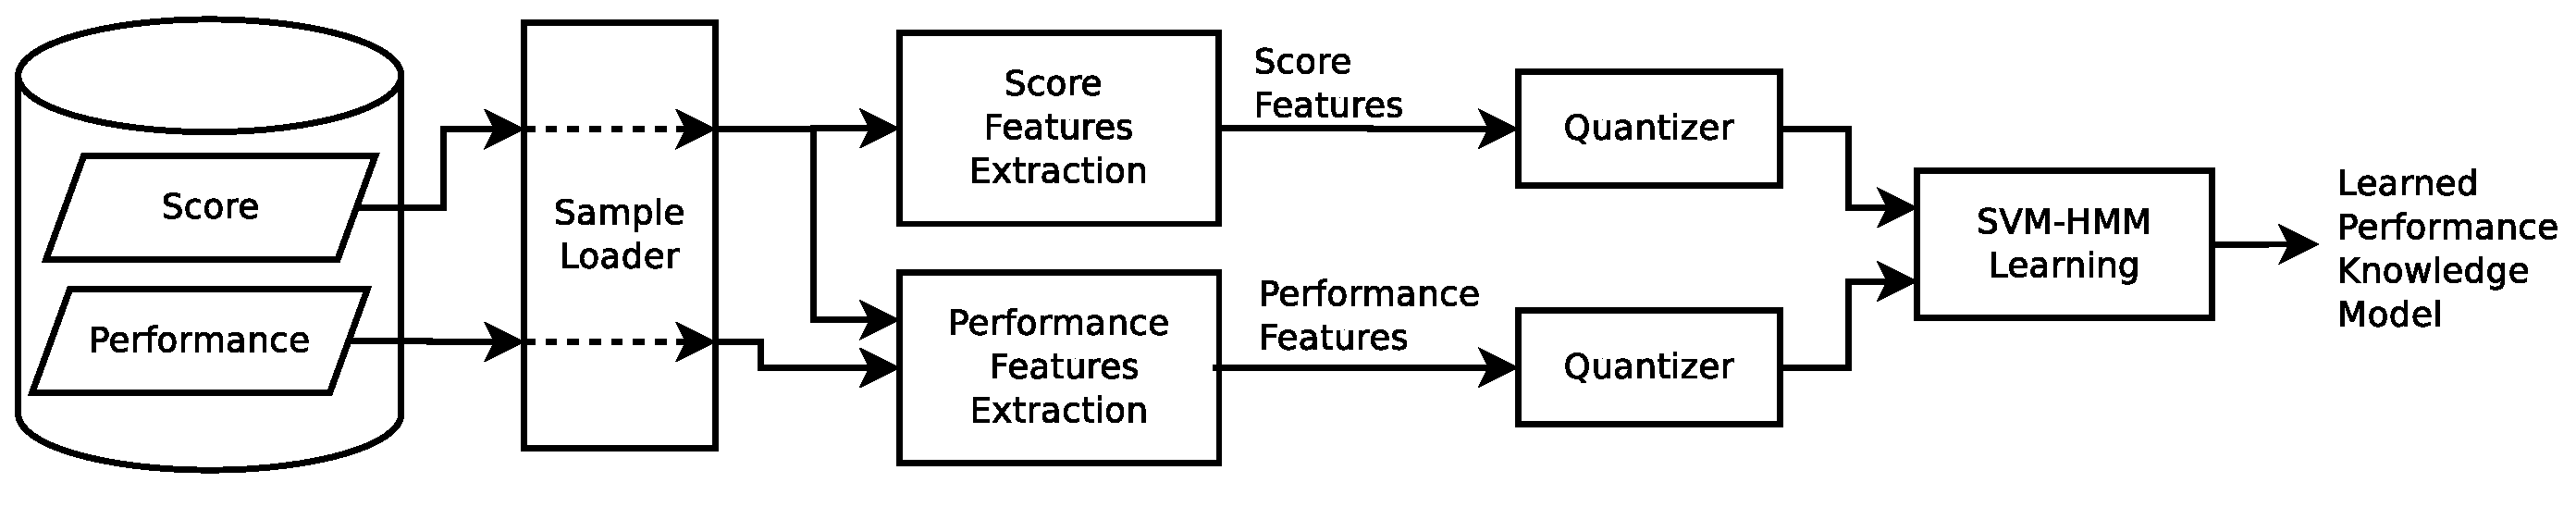
\includegraphics[width=\textwidth]{fig/learn_arch}
   \end{center}
   \caption{Learning phase flow chart} 
   \label{fig:learnflow}
\end{figure*}
The main goal in the learning phase is to extract performance knowledge from training samples. Fig. \ref{fig:learnflow} shows the internal structure of the learning phase.

Training samples are matched score and expressive performance pairs (their format and preparation process is discussed in Chapter \ref{chap:corpus}). The raw data from the samples are too complex to process, so we need to extract important features from them. Two types of features will be extracted from the samples: first, the musicological cues from the scores are called score features; second, the measurable expression from the expressive performances are called the performance features. In order to learn the performance knowledge from the samples, we want to learn a prediction model using SVM-HMM. This process can be analogize to a human performer reading the explicit and implicit cues from the score, and perform the music with certain expressive expression. The definition of the features used will be presented in Section \ref{sec:features}


% The learning module has a input/output interface that is independent of the underlying algorithm, so different algorithm can be implemented without changing the overall structure of the system.

%TODO: sample loader
\subsection{Training Sample Loader}
   A training sample is loaded with the sample loader module, since a training sample is consisted of a score (musicXML format) and an expressive recording (MIDI format), the sample loader finds the two files given the sample name, and load them into an intermediate representation (\texttt{music21.Stream} object provided by the \texttt{music21} librar \cite{music21} from MIT). The music21 library will convert the musicXML and MIDI format into a python Object hierarchy that is easy to access and manipulate by python code. 

One caveat here is that the recording in MIDI may contain very subtle expression. But the music21 library will quantize the MIDI in the time axis by default, which will destroy the subtle onset and duration expression. And the music21 library don't handle the "ticks per quarter note" information in the MIDI heade \cite{midispec}, so we must explicitly specify this value, and explicitly disable quantization during MIDI loading.

\subsection{Features Extraction}
In order to keep the system architecture simple, a feature extractor are designed to be independent to other feature extractors, so features can added or removed without affecting the rest of the system. Furthermore, this enables parallel feature extraction. But sometimes a feature inevitably depends on other features, for example, the \enquote{relative duration with the previous note} is calculated based on the \enquote{duration} feature. Since we want to avoid complex dependency management, the \enquote{relative duration} feature extractor has to calculated the duration itself, instead of depending on the \enquote{duration} extractor. Therefore, the \enquote{duration} feature extracted will be computed twice. To avoid redundant computation of the feature extractors, we implemented a caching mechanism. Once the \enquote{duration} feature had been computed, no matter it is calculated in the \enquote{duration} extractor or in the \enquote{relative dutaion} extractor, it's value will be cached during this execution session, so no matter how many feature extractors uses the \enquote{duration} feature, they can get the value directly from cache. This method can speed up the execution without handling dependencies.

   The extracted features are aggregated and stored into a JavaScript Object Notation (JSON) file for the SVM-HMM module to load. By saving the features in a human-readable intermediate file, we can easily look into the file to debug potential problems.%the learning module can then load this file as inpu.t. The learning algorithm can then do any pre-processing on the features, such as aggregation or quantization. The output of this module is the algorithm specific model description. For example, a linear regression algorithm will output the regression parameters. The algorithm is required to produce a model file containing the model description, but the system doesn't care about the internal format of the model description file, it will simply feed this model file to the generation module in the generation stage. So the developer of the learning module has to implement methods to write and read the model file themselves.

   %In the early stage of this research, linear regression is used. The results of linear regression is shown in \cite{Lyu2012}. In this thesis, Structural Support Vector Machin \cite{Joachims2009} is used instead. The detail of Structural SVM will be in the next Chapter.

\subsection{SVM-HMM Learning}
After all features are extracted, the next step is to learn performance knowledge from the features. In the early stage of this research, we have successfully applied linear regressio \cite{Lyu2012}. However, assuming this problem to be a linear system is clearly an oversimplification. So we switch to structural support vector machine with hidden Markov model output (SVM-HMM)\cite{svm2009, svm2005, svm2003} as our supervised learning algorithm. 

The SVM-HMM learning module loads the feature file from the previous stage, and rearrange the features to fit the required input format of the SVM-HMM learner program. However, most features from the previous stage are real values, but SVM-HMM only takes discrete performance features\footnote{SVM-HMM is initially designed for tasks like part-of-speech tagging, in which real value or binary featrues are used to predict discrete part-of-speech tags.}, so quantization is required. For each performance feature, a quantizer calculates the overall mean and standard deviation from all training samples. There are many possible way to quantize the features, each will result in different output, here we will present a quantizer design for demonstration purpose: a uniform quantizer is employed to quantize a performance feature into 128 intervals/bins. The range between mean minus or plus four standard deviations into 128 uniform intervals. Values over than mean plus four standard deviations are quantized into the 128th bin, and values below mean minus four standard deviations are quantized into the 1st bin. The number of intervals decides how fine-grain the quantization will be, if the number is too low, the quantization error will be too large, expressions across a large range will be quantized into the same bin, and results in dull expression. However, if the number is too large, There will be too few samples for each interval, and the training process will take a lot of CPU and memory resources without significant gain in prediction accuracy. The range of four standard deviation is chosen by trail and error, a narrower range will make most of the extreme values be quantized into the largest of smallest bin, so the performance will have a lot of saturated values. But a very large range will make the interval between each quantization bin too large, rising the quantization error. %Feature values below mean minus three standard deviations are quantized to the lowest bin, while values larger than mean plus three standard deviations are quantized to the highest bin. The range of three standard deviation and 1024 intervals are chosen by experience, which can be modified to fit different corpus. The mean, standard deviation and number of intervals information are stored in a file for the performing phase to dequantize the output.

The theoretical background of SVM-HMM is already mentioned in Section \ref{sec:svm-hmm}. We leverage Thorsten Joachims's implementation called $SVM^{hmm}$ \cite{Joachims2008}. $SVM^{hmm}$ is an implementation of structural SVMs for sequence tagging \cite{svm2003} using the training algorithm described in \cite{svm2005} and \cite{svm2009}. The $SVM^{hmm}$ package contains a SVM-HMM training program called \texttt{svm\_hmm\_learn} and a prediction program called \texttt{svm\_hmm\_classify}, which will be used in the performing phase. For structural simplicity, we train one independent model for each performance feature, each model uses all the score features to try to predict a single quantized performance feature. The \texttt{svm\_hmm\_learn} takes a training file describing those features. Each line represents features for a note, organized in the following format:
\begin{lstlisting}
	PERF qid:EXNUM FEAT1:FEAT1_VAL FEAT2:FEAT2_VAL ... #comment
\end{lstlisting}
\texttt{PERF} is a quantized performance feature. The \texttt{EXNUM} after \texttt{qid:} identifies the phrases, all notes in a phrase will have the same \texttt{qid:EXNUM} identifier. Following the identifier are quantized score features, denote as \texttt{feature name : feature value}, separated by spaces. And anything after a \texttt{\#} symbol is comment. %An example of the training file is shown in Fig. \ref{fig:expinput}

\framebox{TODO: partial model}

%\begin{figure*}[tp]
%   \begin{center}
%      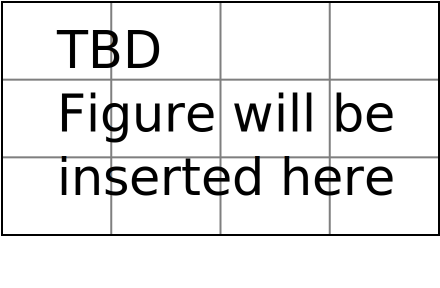
\includegraphics[width=\textwidth]{fig/TBDFigure}
%   \end{center}
%   \caption{Example input file} 
%   \label{fig:expinput}
%\end{figure*}

There are some key parameters needed to be specified for the training program. First the $C$ parameter in SVM, which controls the trade-off between lowering training error and maximizing margin. Larger C will result in lower training error, but the margin may be smaller. Second, the $\varepsilon$ parameter controls the required precision for termination. The smaller the $\varepsilon$, the precision should be higher, but may require more time and memory resource to compute. Finally, for the HMM part, we need to specify the order of dependencies of transition states and emission states. In our case, transition dependency is set to one, which stands for first-order Markov property, and emission dependency is set to zero. Since we train separate models for each performance feature, each model can have their own set of parameters. The parameter selection process is done by experiment, which will be presented in Chapter \ref{chap:exp}

Finally, the training program will output three model files (because we use three performance features). In the model file are the SVM-HMM model parameters, such as the support vectors and other metadata. Since it takes considerable time (roughly a dozen minutes or to a few hours) to train a model (depending on the amount of training samples and the power of the computer running the system), the system can only support off-line learning. But the learning process only need to be run once. The performance knowledge model can be reused over and over again in the performing phase.



\section{Performing Expressively}
   \begin{figure*}[tp]
      \begin{center}
         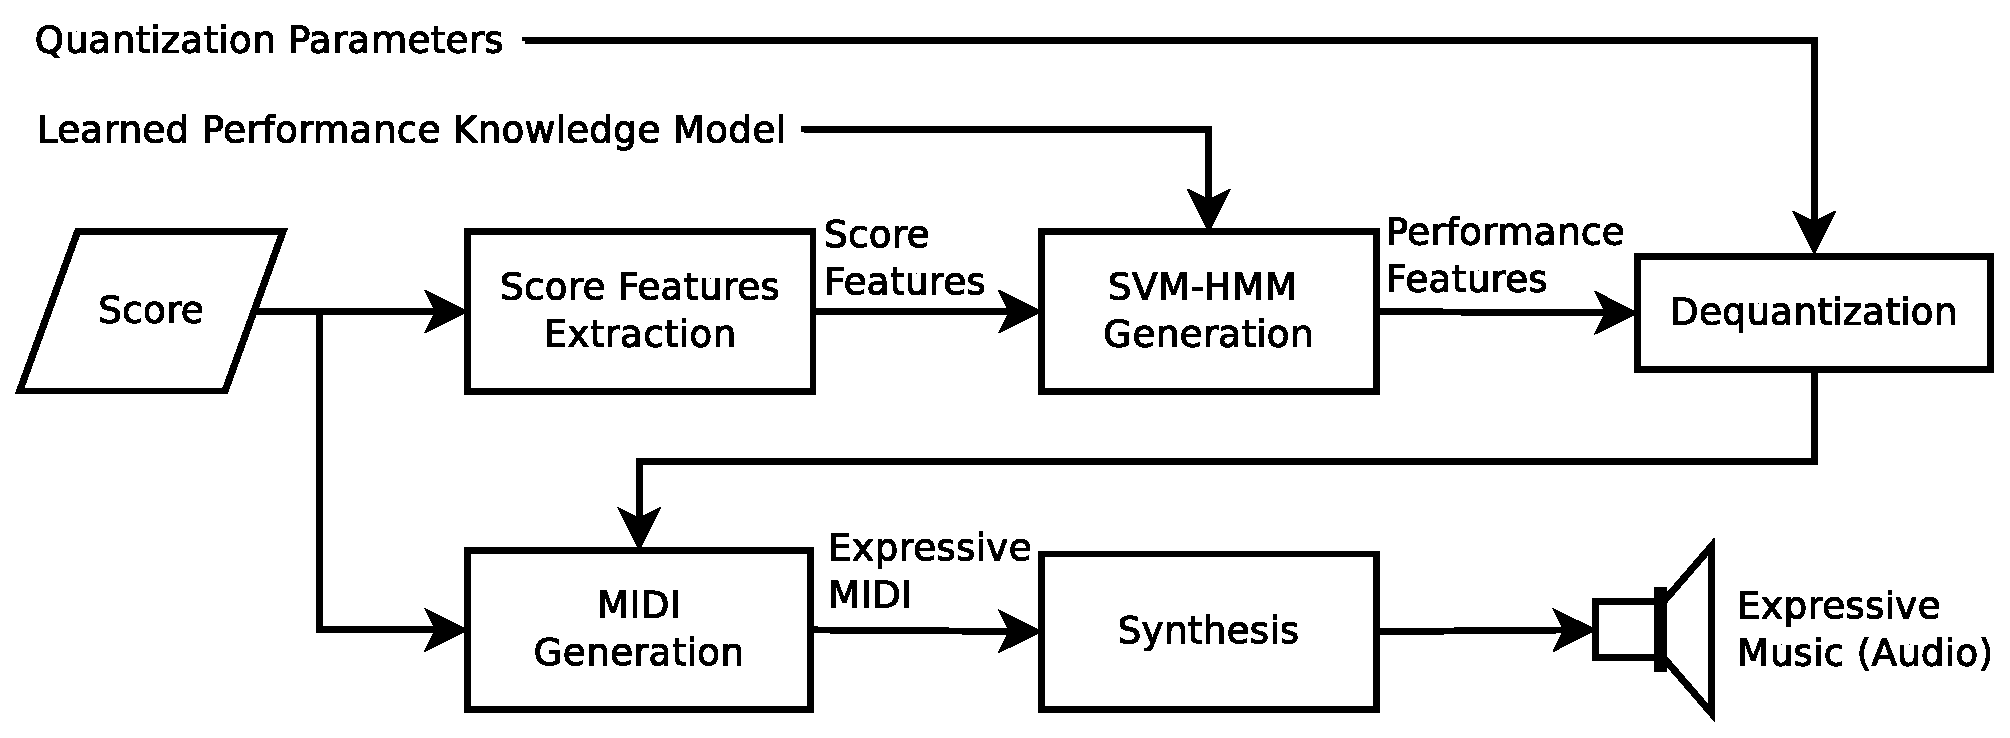
\includegraphics[width=\textwidth]{fig/perf_arch}
      \end{center}
      \caption{Performing phase flow chart} 
      \label{fig:perfflow}
   \end{figure*}
The performing phase uses the performance knowledge model learned in the previous phase to generate expressive performances. The input is a score file, which should not be used during training to prevent overfitting. Score features will be extracted from it using the same code as in the learning phase. The SVM-HMM generation module will use the learned model and the score features to predict the performance features. These features will than be de-quantized back to real values using the method described previously. An MIDI generation module will apply those performance features onto the score to produce a expressive MIDI file. The MIDI file itself is already a expressive performance, in order to listen to the sound, an software synthesizer can be used to render the MIDI file into WAV or MP3 format.
\subsection{SVM-HMM Generation}
The feature extraction and aggregation process in the performing phase is similar to the learning phase, but the \texttt{PERF} fields in the SVM-HMM input file are all set to zero, meaning that we don't know its value and wish the algorithm to predict it. The \texttt{svm\_hmm\_classify} program will take these inputs with the learned model file and predict the quantized labels of the performance features. These performance features are de-quantized back to real values. When reconstructing the features from the quantized value during the performing phase, the middle point of each bin is used. For the 128th bin, the mean plus four standard deviation is used, and similarly for the 1st bin, the mean minus four standard deviation is used.
%If we already know the real performance feature value, say, we use part of the corpus as training set and the rest as testing set, the \texttt{PERF} can be set to the \enquote{answer} of the testing set, so the \texttt{svm\_hmm\_classify} program will calculate the accuracy of the prediction. 

      
\subsection{MIDI Generation}
  %Since the output of the SVM-HMM learner is the quantized label for the performance feature, dequantization is required to turn those values back to real-valued performance features. The dequantizer will load the quantization parameters from the learning stage to understand the range and intervals used in the quantizer. Each quantization label is dequantized into the mean value of the interval it belongs.

The performance features are than applied onto the input score. The onset timings will be shifted, the duration extended or shortened, and the loudness shifted according to the predicted performance features. The resulting expressive performance will be transfromed into MIDI files using \texttt{music21} library.%For example, if a performance feature represents the note's duration should last for 1.2 times of its nominal value, the duration in the score is multiplied by 1.2. After all the performance features are applied, the expressive version of the score is stored in MIDI format using the \texttt{music21} library.

\framebox{TODO:Dramatization/post processing}
\subsection{Audio Synthesis}
In order to actually hear the expressive performance, the MIDI file can be rendered by a software MIDI synthesizer. %Since the output is standard MIDI file, the user can choose any compatible software or hardware synthesizer. 
Such as \texttt{timidity++} software synthesizer for Linux. The output will be an WAV (Waveform Audio Format) file, which can be compressed into MP3 (MPEG-2 Audio Layer III) by \texttt{lame} audio encoder. Alternatively, one can use hardware synthesizers, for example, RenCo \cite{RenCon} contest uses Yamaha Disklavier Digital Piano to render contestants' submission.

Because sub-note-level expression is not the primary goal of this research, we choose standard MIDI grand piano sound to render the music. The system can be extended to used more advanced physical model or musical instrument specific audio synthesizer. Sub-note level features, such as special techniques for violins, can be added to the features list and be learned by the SVM-HMM model.
   
\framebox{TODO: phrase concatenation}
\framebox{REVIEW1}
\section{Features}\label{sec:features}

   %The system is trying to mimic the process of human performance: the musican reads the explict and implict cues from the score and transform them into musical expressions. So the features can be categorized into two category: score features and performance features. Score features are information contained in the score. Performance features corresponds to the musical expression. The basic time unit for both features are a note. 
   As mentioned in Section \ref{sec:learn}, there are two types of features, score features and performance features. We will present the features used in the system, and discuss the difficulties encountered.
\subsection{Score Features}
      Score features are musicological cues presented in the score. The purpose of score features are to simulate the high level information a performer may perceive when he/she reads the score. The basic time unit for the features are notes. Each note will have one of each features presented below.
      Score features includes:
      \begin{description}
         \item [Relative position in a phrase:]
            The relative position of a note in the phrase, its value ranges from 0\% to 100\%. %Since there are often salient musical expressions during the opening or closing of a phrase, this feature is used to capture the start or end of the phrase.
            This feature is intended to capture the special expression in the start or the end of a phrase, or to capture time-variant expression like arch-type loudness variation.
         \item [Relative pitch:]
            The pitch of a note relative to the pitch range of the phrase, denoted by MIDI pitch number (resolution is down to semitone). For a phrase of $n$ notes with pitch $P_1, P_2, \dots, P_n$, $$RP = \frac{P_i -min(P_1, P_2, \dots, P_n) }{max(P_1, P_2, \dots, P_n)-min(P_1, P_2, \dots, P_n) }$$  Where $P_i$ is the pitch of note at position $t$.

         \item [Interval from the previous note:] The interval between the current note and its previous note (in semitone). This represents the direction of the melodic line. $$IP = P_{i} - P_{i-1} $$ See Fig. \ref{fig:interval} for example.
         \item [Interval to the next note:] The interval between the current note and its previous note (in semitone). $$IN = P_{i+1} - P_i$$ See Fig. \ref{fig:interval} for example.
         
      \begin{figure}[tp]
         \begin{center}
            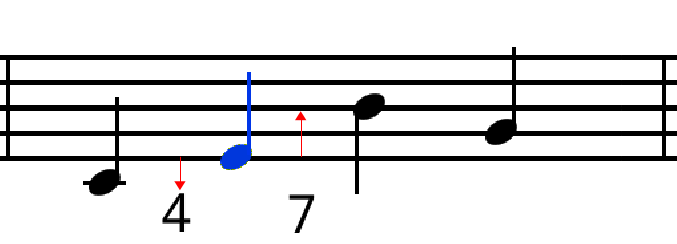
\includegraphics[width=0.4\textwidth]{fig/interval_arrow}
         \end{center}
         \caption{Interval from/to neighbor notes}
         \label{fig:interval}
      \end{figure}

         
         \item [Note duration:] The duration of a note (quarter notes). 

            Grace notes have zero duration in musicXML specification. The reason for this is that grace notes are considered very short ornaments that does not occupy real beat position. But zero duration is hard to handle in math formulation. So we assigned a duration of $\frac{1}{64} = 0.0625$ quarter note to all grace notes, which is equivalent to the length of a sixty-fourth note. Sixty-fourth note is chosen because it's far shorter than all the notes in our corpus.
         \item [Relative Duration with the previous note:] The duration of a note divided by the duration of its previous note. For a phrase of $n$ notes with duration $D_1, D_2, \dots, D_n$, $$RDP = \frac{D_i}{D_{i-1}} $$ See Fig. \ref{fig:duration} for example.
            This feature is intended to locate local change in tempo, such as a series of rapid consecutive notes followed by a long note, which will cause a discontinuity in this feature.
         \item [Relative duration with the next note:] The duration of a note divided by duration of its next note. $$RDN = \frac{D_i}{D_{i+1}} $$ See Fig. \ref{fig:duration} for example.

      \begin{figure}[tp]
         \begin{center}
            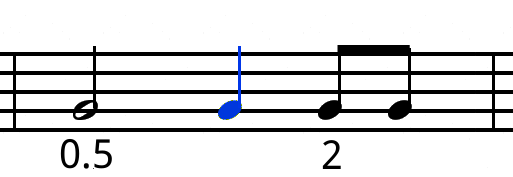
\includegraphics[width=0.4\textwidth]{fig/duration}
         \end{center}
         \caption{Relative duration with the previous/next note}
         \label{fig:duration}
      \end{figure}
   \item [Metric position:] The position (beat) of a note in a measure. For example, a $^4_4$ time signature will have a beat unit of a quarter note. So if the measure consists of four quarter notes, each of them will have metric position of 1, 2, 3 and 4. Please refer to Fig. \ref{fig:metrical} for example.
      
      Metric position usually implies beat strength. In most tonal music, there exist a hierarchy of beat strength. For example, in a measure of a $^4_4$ piece, the first note is usually the strongest, the third note is the second strongest, and the second and fourth notes are the least strong.

   \begin{figure}[tp]
      \begin{center}
         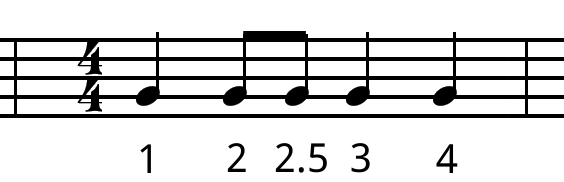
\includegraphics[width=0.4\textwidth]{fig/metrical}
      \end{center}
      \caption{Metric position}
      \label{fig:metrical}
   \end{figure}
      \end{description}

      %TODO: link to narmour group
%   \begin{figure*}[tp]
%      \begin{center}
%         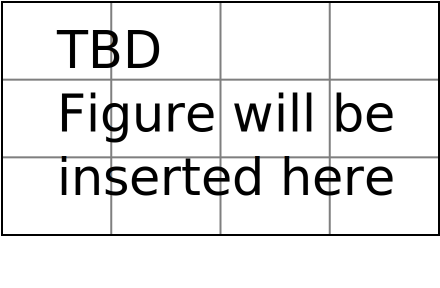
\includegraphics[width=0.8\textwidth]{fig/TBDFigure}
%      \end{center}
%      \caption{Example Score Features}
%      \label{fig:expScoreFeat}
%   \end{figure*}



\subsection{Performance Features}
   Performance features are the expressions we would like to learn from a performance. Performance features are extracted by comparing the expressive performance with the score.
      Performance features includes:
      \begin{description}
         \item [Onset time deviation:] 
            The onset time of a natural human recording will not be exactly on the beat, this phenomenon is roughly corresponding to the music term \enquote{rubato.} The onset time deviation is the difference of onset timing between the performance and the score. Namely,
            $$ ROB = O_i^{perf} - O_i^{score} $$ Where $O_i^{perf}$ is the onset time of note $i$ in the performance, $O_i^{score}$ is the onset time of note $i$ in the score. 

            However, the above formula assumes the performance is played at the exact same tempo as assigned in the score. In the corpus we use, test subject can't always keep up with the speed of the score because of limited piano skill, or they may speed up or slow down certain sections as their expression. Therefore, the performance should be linearly scaled to avoid systematic bias, We will discuss this issue in Section \ref{sec:normalize}.
         \item [loudness:] The loudness of a note. Measured by MIDI velocity level 0 through 127.
            $$ RL = \frac{L_i}{max(L_1, L_2, \dots, L_n)}$$

         \item [Relative duration:]
            The performed duration of a note divided by the nominal duration on the score.
            $$ RD = \frac{ D_i^{perf}}{D_i^{score}}$$
      \end{description}

%\begin{figure*}[tp]
%   \begin{center}
%      %TODO:Fig.:Example JSON code
%      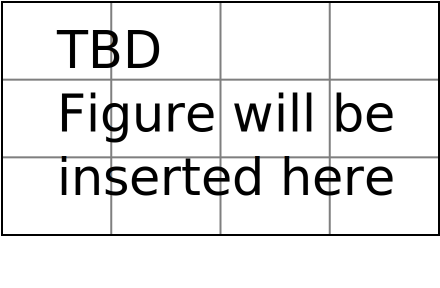
\includegraphics[width=\textwidth]{fig/TBDFigure}
%   \end{center}
%   \caption{Example Performance Features}
%   \label{fig:expPerfFeat}
%\end{figure*}
   % \section{Melodic Similarity and Sample Selection}
   % Once a score is given to the system for playing, all the samples in the database will be ranked by the melodic similarity with the given score. Here we use the melodic distance function provided by the MIDI Toolbo \cite{Eerola2004}, which is defined as follows: 
   % \begin{enumerate}
   %    \item Melodic contour is calculated by connecting each note's pitch, forming a piece-wise linear contour.
   %    \item Subtract the contour by it's mean to preserve only the relative part.
   %    \item If the two phrases has different length, re-sample both phrases with fixed intervals so both of the phrase will have contour vector of the same length.
   %    \item The L1 norm (a.k.a Taxicab distance) of these two contour vector is the similarity measure. 
   % \end{enumerate}
   % The reason I choose melodic contour is because it yields best results in finding melodic similarity, which is shown in \cite{Hoffmann-engl2005}.

      %TODO: not included features: e.g. notation
   \subsection{Normalizing Onset Deviation}
   \label{sec:normalize}
\begin{figure}[tp]
   \begin{center}
      %TODO:Fig.:Normalization Schemes
      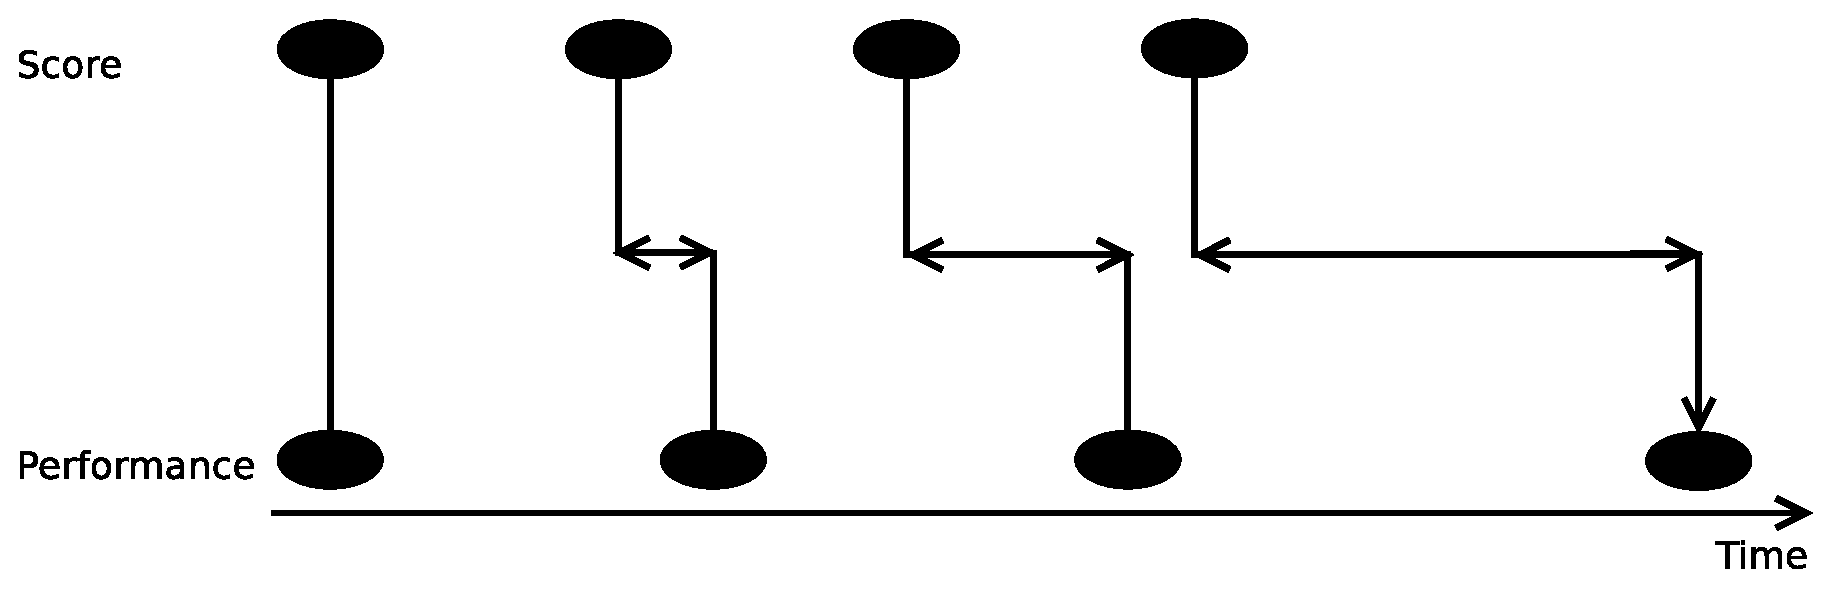
\includegraphics[width=\textwidth]{fig/prob_onset_diff}

   \end{center}
   \caption{Systematic bias in onset deviation }
   \label{fig:normalizationprob}
\end{figure}
%\begin{figure}[tp]
%\begin{center}
%%TODO:Fig.:Normalization Schemes
%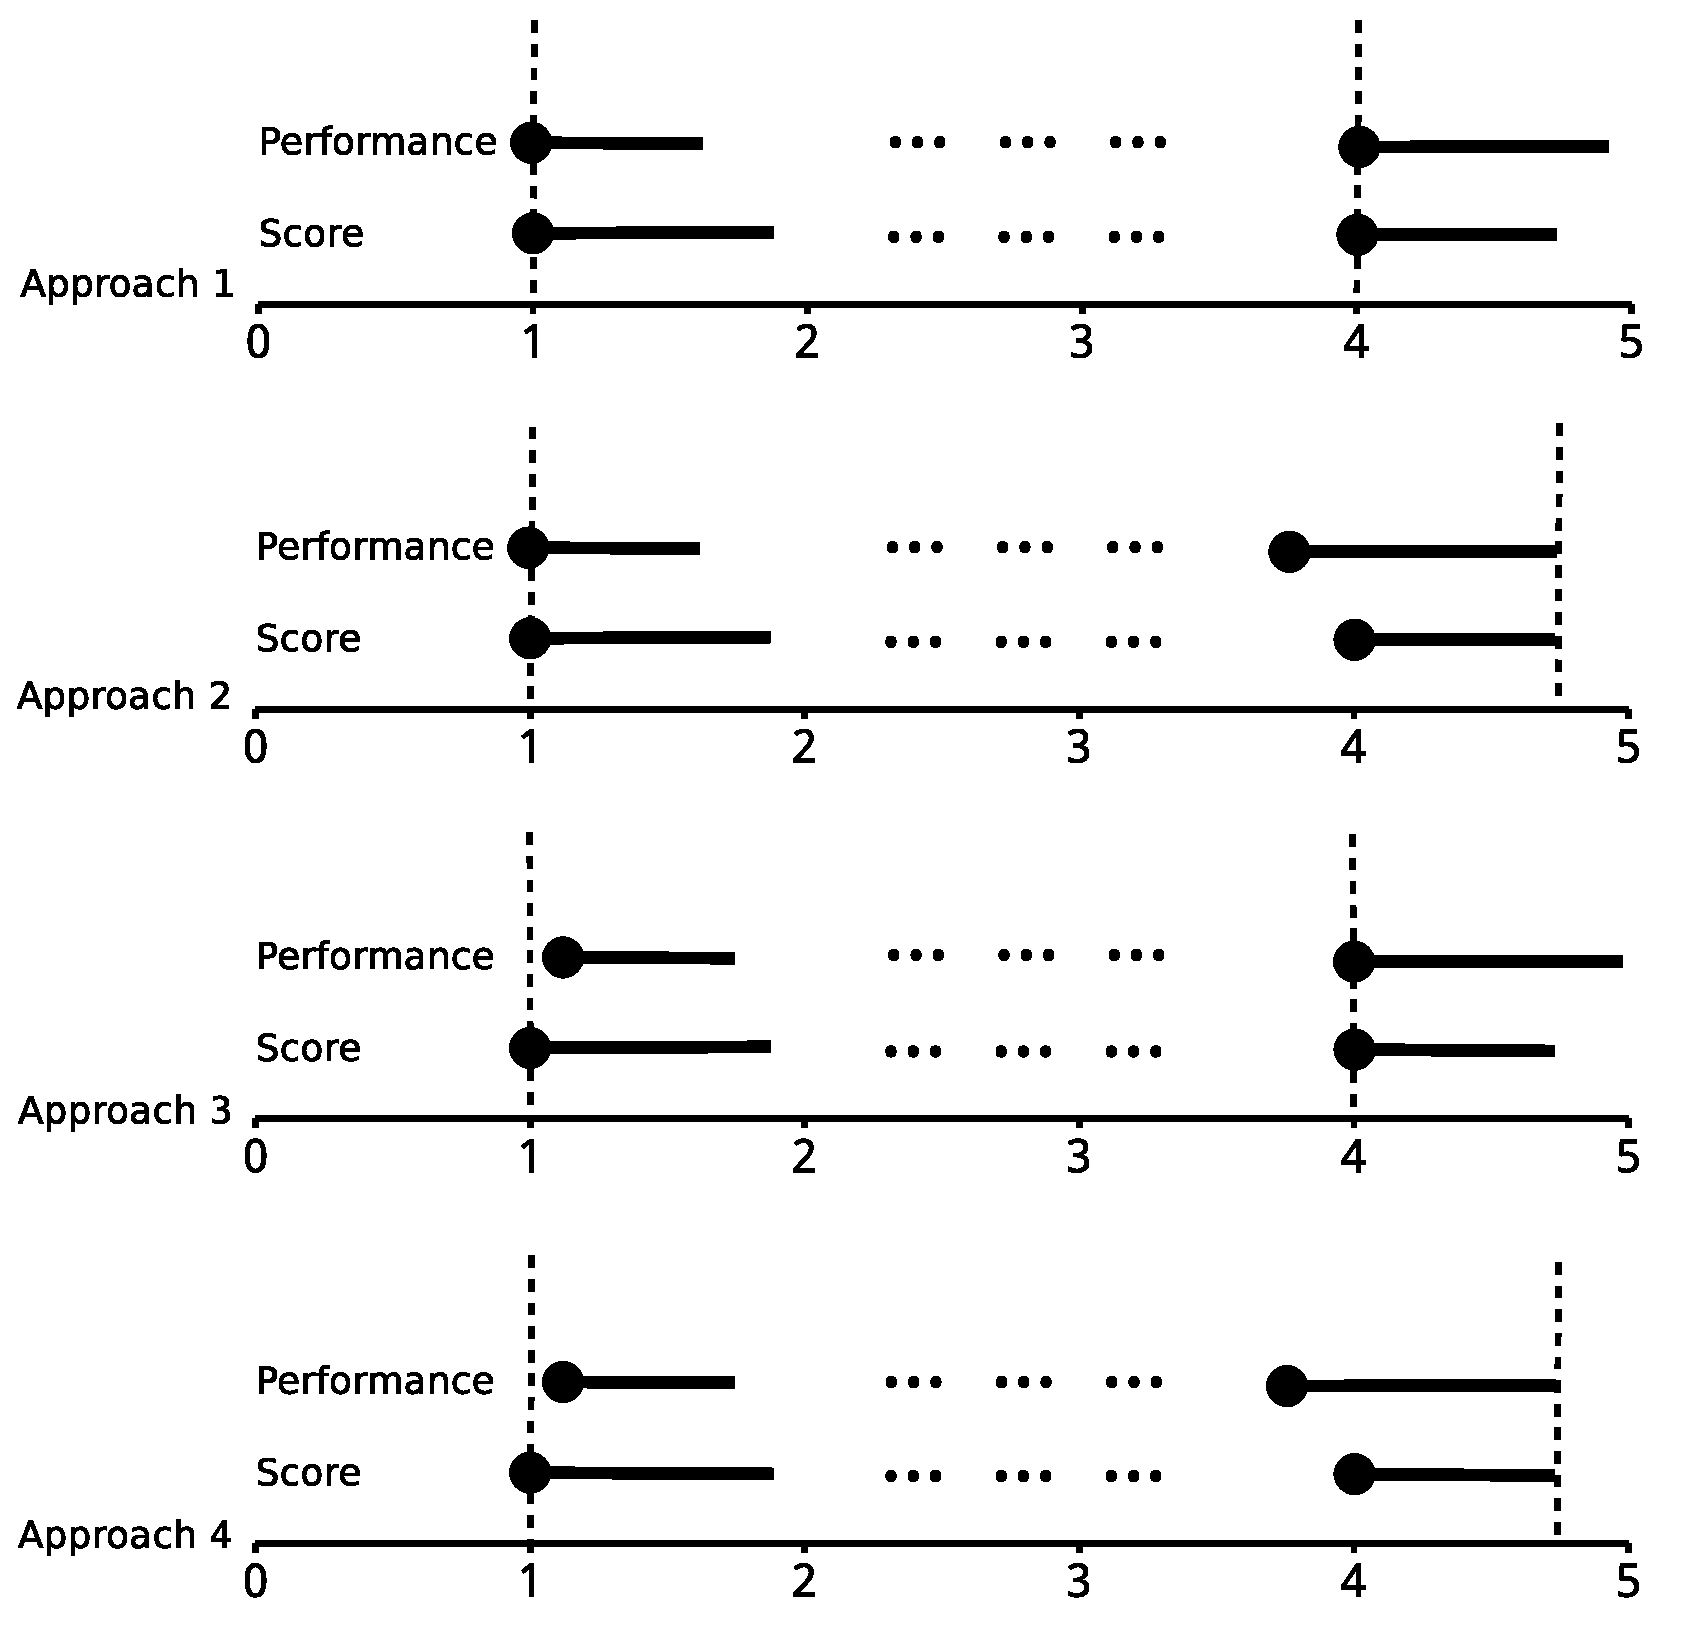
\includegraphics[width=\textwidth]{fig/onsetdifffix}
%
%\end{center}
%\caption{Normalization Schemes}
%\label{fig:normalization}
%\end{figure}
In th previous section, we mentioned that the onset deviation feature will have problem when performance is not played at the exact temp indicated on the score. As illustrated in Fig. \ref{fig:normalizationprob}, if the performance is played faster than expected, the deviation will grow larger and larger over time. The systematic bias caused by the difference in total duration will mix up with the local note deviation, For a long phrase, the onset deviation of the last notes can larger than a dozen quarter notes. These kind of extreme values will cause erroneous predictions in the model: a note may be delayed for a very large deviation, causing it to be played after the next note, the swapped notes will destroy the melody.
 
In other words, the original definition of the onset deviation actually contains two type of deviation: a global/systematic deviation cause by the difference between performed and nominal tempo, and a local deviation cause by note-level expression. Since the intention of the onset deviation features is to catch the note-level expression, the performance must be linearly scaled to cancel the global deviation.

%The relative onset deviation feature must be normalized to get meaningful result. For example, a phrase is played very fast by the performer, say, the played length is only 70\% of the notation. If the first note is aligned, the onset timing bias will grow linearly until the end of the phrase, the last note will have a onset timing bias of about 30\% of the phrase. But from the definition of this feature, the timing bias should be roughly less than half of  a note's length, and it's mean should be around zero. This 30\% value will introduce a relative large value in the training corpus, and thus there may be very large output value from the generation phase. If the model predict that a note should be played early or later for 30\% of the phrase length, the melody will be messed up. 

   Initially, we tried two possible type of normalization methods : 
   \begin{enumerate}
      \item Align the onset of the first notes, align the onset of the last notes
      \item Align the onset of the first notes, align the end of the last notes
      %\item Don't align the onset of the first notes, align the onset of the last notes
      %\item Don't align the onset of the first notes, align the end of the last notes
   \end{enumerate}
    %The incentive for not aligning the first note is that the performer may intend to use an early start or delayed start as an expression, if the first note is aligned by it's onset, the first note in every phrase will have a onset timing bias feature of value zero. In other words, the early/delayed start expression is lost. %But each normalization method are equally reasonable theoretically, so we need to use empirical data to verify them. The experiment is explained in section \ref{TODO:experiment}. The experiment result showed that [TODO: result]
   We proposed an automated approach to find the best scaling ratio to address this problem. First we have to define the distance between scaled phrases as our target to minimize. If we represent a phrase as a vector of all the onset timings, the $l^2$-norm of the tow vectors can be treated as the distance. Note that the two vectors must have the same size, because the recordings are required to match note-to-note with the score. Using this distance measure, we would like to find an optimal scaling ratio such that the scaled recording has the minimum distance from the score. Brent's Metho \cite{brent1973} is used to find the optimal ratio. To speed up the optimization and prevent unreasonable value, a search range of $[initial\ guess \times 0.5 , initial\ guess \times 2]$ is imposed on the optimizer. The $initial\ guess$ is used as a rough estimate of the ratio, calculated by aligning the first and last onset of the phrase. Than we assume the actual ratio will not be smaller than half of $initial\ guess$ and not larger than twice of $initial\ guess$. The two numbers 0.5 and 2 are chosen by trail and error, but most of the empirical data suggest is valid most of the time. We will demonstrate the effectiveness of this solution in Section \ref{sec:onsetnormexp}

   %So we have defined a automatic method to dynamically adjust the normalization ratio to eliminate systematical error in the onset deviation feature. Comparing this method to not using any normalization (see Fig. \ref{fig:afternorm}), the method can produce very low onset deviations, roughly centered around zero, while the result from not using any normalization will show a clear trend of increasing deviations.
 

